\section{Aufbau}
Eine Skizze des Aufbaus ist in Abbildung \ref{fig:schem_auf} zu sehen. Das Michelson-Interferometer besteht  aus einem Strahlteiler, der den eintreffenden Strahl in zwei Teilstrahlen teilt. Die Teilstrahlen werde jeweils von einem Spiegel reflektiert. Einer der der beiden Spiegel kann �ber einen Hebelmechanismus, durch einem Elektromotor mit nahezu konstanter Geschwindigkeit bewegt werden. Der reflektierte Strahl wird durch eine CaF$_2$-Sammellinse auf eine pyroelektrischen Detektor geworfen. Der Detektor wandelt den Strahl in eine Spannung proportional zur Intensit�t des Strahls um. Die Spannung wird mit einem Lock-In-Verst�rker bearbeitet und �ber ein AD-Box an den Computer weitergeleitet. Am Computer wird aus dem Signal mit der Software Lab-View ein Interferogramm visualisiert. 
Das �bersetzungsverh�ltnis k des Hebelmechanismus, f�r den Gangunterschied liegt bei ca. 5 (Quelle:\cite{Staatsex_Michels}). Da der Teilstrahl, der auf den bewegten Spiegel trifft das Medium des Strahlteilers drei mal durchqueren muss, wird zwischen dem Strahlteiler und dem festem Spiegel noch ein Kompensationspl�ttchen angebracht.
Als Strahlenquelle wird ein HeNe-Laser und ein Muffelofen verwendet. Der Laser hat eine Wellenl�nge von \SI{3,39}{$\mu$m}, der Muffelofen und der Laser k�nnen �ber den Folienspiegel gekoppelt werden. Zwischen dem Muffelofen und dem Folienspiegel ist ein Chopper eingebaut, der die Spannung des Detektors regelt. Durch den Chopper registriert der Detektor immer die Temperatur- und Strahlungs�nderung (Untergrund) und die zu messende Strahlung (mit Untergrund) abwechselnd. Die Trennung der beiden Signal wird mittels eines phasenempfindlichen Lock-In-Verst�rker und eines anhand Referenzsignals vorgenommen. Der Muffelofen kann bis 900$^\circ$C erhitzt werden, die dabei emittierte Strahlung durch eine Blende kollimiert. Es kann ein Schmalbandfilter verwendet werden, um die Wellenl�nge der Strahlung aus dem Muffelofen auf einen Bereich um ca. \SI{3,31}{$\mu$m} zu begrenzen.

\begin{figure}[H]
\centering
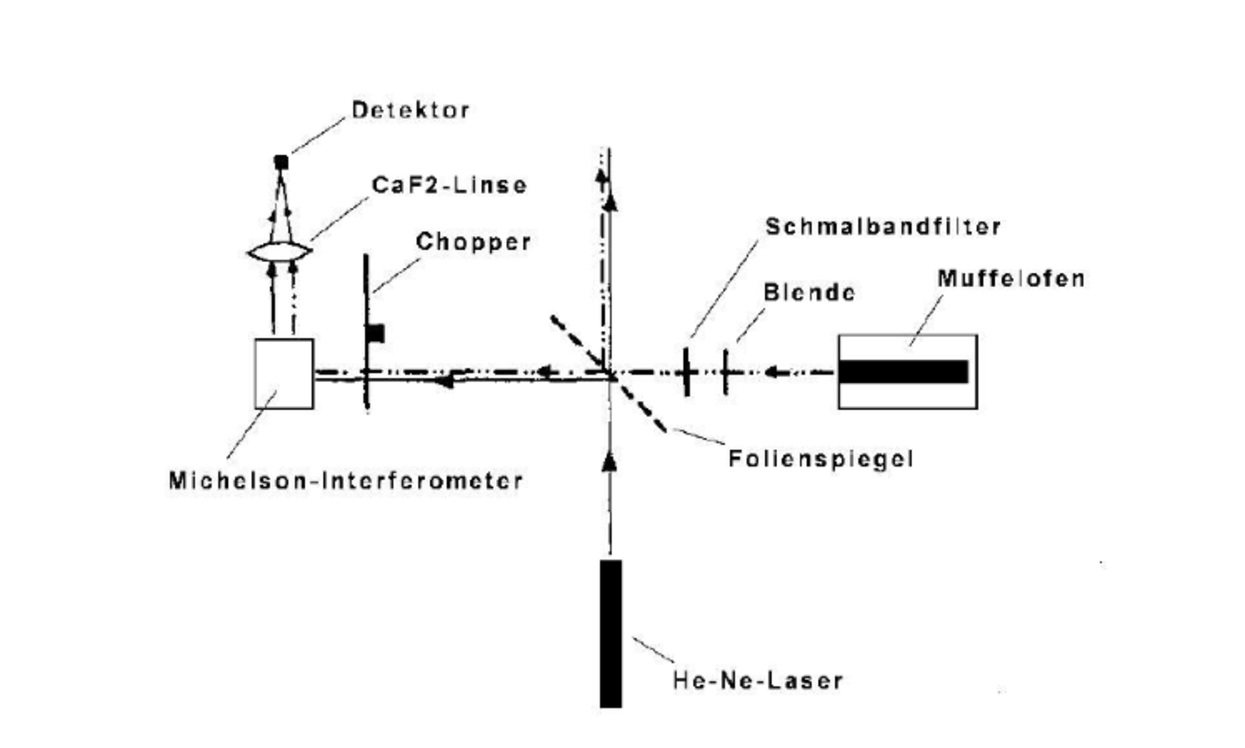
\includegraphics[scale = 1,trim = 3cm 0cm 3cm 0cm]{Schematischer_Aufbau_Michelson}
\caption{Aufbau des Experimentes \cite{Schematischer_Aufbau}}
\label{fig:schem_auf}
\end{figure}

\subsection{Pyroelektrischer Detektor}
Pyroelektrische Detektoren (vgl. \cite{pyroel_detek}) bestehen aus ferroelektrischen Kristallen oder Keramiken mit unsymmetrischer Gitterstruktur, deren Gitterabst�nde sich bei Erw�rmung durch IR-Stahlung ver�ndern. Das Meterial hat dadurch temperaturabh�ngige Dipolmomente, welche es polarisieren. Die �nderung der Polarisation resultiert in einem elektrischen Signal, welches f�r Temperaturen im Bereich der Raumtemperatur n�herungsweise proportional zur �nderung der Strahlungsleistung ist. Der schematische Aufbau ist in Abb. \ref{fig:pyro_detek} dargestellt. In diesem Versuch ist die Detektorspannung abh�ngig von der Chopperfrequenz, welche die einfallende Strahlung periodisch unterbricht. Bei hoher Chopperfrequenz wird die Spannung kleiner.
\begin{figure}[H]
\centering
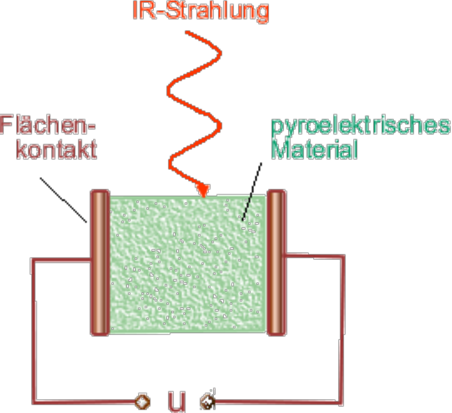
\includegraphics{pyro_m35bi0101.pdf}
\caption{Aufbau eines pyroelektrischen Detektors \cite{pyroel_detek}}
\label{fig:pyro_detek}
\end{figure}
